\documentclass[12pt]{article}

\usepackage{sbc-template}

\usepackage{graphicx,url}

%\usepackage[brazil]{babel}   
\usepackage[latin1]{inputenc}  
\usepackage{multirow}
     
\sloppy

\title{Um estudo exploratório sobre o uso das ferramentas educacionais no Ambiente Virtual de Aprendizagem Moodle}

\author{Marcelo A. Santana\inst{1}, Baldoino S. Neto\inst{1}, Evandro B. Costa\inst{1} }


\address{Instituto de Computação -- Universidade Federal de Alagoas
  (UFAL)\\
  Maceió-- AL -- Brasil
}

\begin{document} 

\maketitle

\begin{abstract}
   .....
\end{abstract}
     
\begin{resumo} 
A Educação a distância vem sendo cada dia mais utilizada pelas instituições de ensino, tanto para apoio aos cursos presenciais como para cursos à distância. Nesse cenário, uma ferramenta muito importante é o AVA. Este estudo tem como objetivo principal avaliar o uso dos recursos e ferramentas disponível no AVA Moodle. Para realização deste trabalho foram utilizadas técnicas de mineração de dados e aplicado um questionário aos tutores online.Após análise dos experimentos realizados, os resultados apontam que muitas das ferramentas disponíveis estão sendo subutilizadas pelos professores, tutores e estudantes.
\end{resumo}


\section{Introdução}

A educação a distância está crescendo rapidamente em todo o mundo. Um dos principais métodos de ensino à distância desenvolvido é o que usa a internet como meio de comunicação. Para isso, precisa-se de um Ambiente Virtual de Aprendizagem (AVA) \cite{Magalhaes:2010:IDU:1999593.1999626}. Que pode oferecer uma grande variedade de canais e espaços de trabalho para facilitar o compartilhamento de informação e comunicação entre os participantes de um curso. Eles permitem que os educadores distribuam informações para os alunos, produzam material de conteúdo, prepararem trabalhos, testes, se envolvam em discussões, gerenciem classes à distância e permitem a aprendizagem colaborativa com fóruns, chats, áreas de armazenamento de arquivos, serviços de notícias, etc \cite{journals/ce/RomeroVG08}. Hoje em dia, um dos AVAs mais utilizado no mundo é o Moodle (objeto modular orientada ambiente de aprendizagem do desenvolvimento), que é uma plataforma de aprendizagem projetada para fornecer aos educadores, administradores e alunos um sistema robusto, seguro e integrado para criar ambientes de aprendizagem personalizados \cite{Moodle:2014}.

Existem vários tipos de atividades que os professores podem colocar em prática em cursos a distância. No entanto, a viabilidade dessas atividades ainda está ligada a ferramentas ``tradicionais'' e pouca atenção é dada à discussão se eles são apropriados para a tarefa e, se não, oque poderia ser melhorado \cite{Oeiras:2006:DDF:1298023.1298032}. Será que realmente todos esses recursos estão sendo utilizados? Será que os professores estão usando esses recursos de forma correta? Quais as ferramentas mais utilizadas? Quais ferramentas de fato são uteis para o processo de ensino e aprendizagem dos estutantes?

Este estudo tenta responder algumas dessas perguntas, a forma de responder essas perguntas foi utilizando dois métodos. O primeiro foi aplicar um questionário aos tutores para identificar quais ferramentas eles mais usam e quais dificuldades encontradas por eles ao usar essas ferramentas. O segundo método foi usar uma característica do moodle que é a de manter registros detalhados de todas as atividades que os alunos realizam, gerando grandes quantidades de dados. Toda esta informação gerada fornece uma ``mina de ouro'' de dados educacionais que podem ser usados para analisar a viabilidade dos recursos disponibilizados. E para analisar essas grande quantidade de dados foi utilizada técnicas de mineração de dados.  

Um dos principais desafios em trabalhar com grandes quantidades de dados é ser capaz de extrair o conhecimento que está implícito nas bases de dados e os tornarem úteis para as pessoas envolvidas. Técnicas de mineração de dados podem ser aplicadas para analisar um grande volume de dados gerados em AVAs. Este procedimento é chamado EDM (Educational Data Mining). EDM está preocupado com o desenvolvimento de métodos para explorar os dados em ambientes educacionais e, através destes métodos, entender melhor os alunos e os contextos em que eles aprendem \cite{baker2010data}.

Para realização do estudo, foi nescessário auxilio de uma ferramenta para extração, transformação e carga de dados e outra para aplicar os algoritmos de mineração de dados. As ferramentas escolhidas foram Pentaho Data Integration e Weka ambos os softwares são livre.

\section{Metodologia}

Objetivando entender se ferramentas e recursos presentes dentro do ambiente virtual de aprendizagem Moodle realmente estão sendo utilizadas e se influenciam no desempenho dos estudantes, foi realizado um estudo exploratório utilizando técnicas de EDM e aplicado um questionário para os tutores online para identificar a relação entre as ferramentas utilizadas e o desempenho dos estudantes. 

A plataforma Moodle permite à transmissão e organização dos conteúdos com auxilio dos seus recursos e ferramentas, facilitando a comunicação síncrona e assíncrona, esses recursos estão divididos em dois. Os estáticos (páginas web, páginas de texto e conteúdo de pastas) e os dinâmicos (chat, diário, fórum glossário, wiki, livros, etc.). O estudo foi realizado sobre as ferramentas dinâmicas: Modulos, assing, blog, book, chat, choice, discussion, fórum, glossary, message, quis, survey e wiki. Essas ferramentas foram escolhidas por serem ferramentas onde ocorre a maior interação entre o professor/tutor e os estudantes.
Seguidos os procedimentos metodológicos foram criadas algumas etapas como segue abaixo:
\begin{enumerate}
\item	Pesquisa bibliográfica sobre Ambientes Virtuais de Aprendizagem, Mineração de dados e Mineração de dados na Educação (EDM);
\item Elaboração de um questionário para os tutores para identificar quais ferramentas são mais usadas pelos tutores e estudantes. 
\item Seleção e tratamentos dos dados, objetivando preparar os dados para aplicação de técnicas de EMD;
\item Realização dos experimentos.
\end{enumerate} 
Desenvolvida essas etapas, foi possível identificar se os tutores online estão muito atarefados, quais as ferramentas mais utilizadas e qual a relação das ferramentas com o desempenho dos estudantes. Os principais resultados e considerações sobre as etapas acima são apresentadas na seção 6.

\section{Trabalhos relacionados}
Pesquisando os trabalhos na área de Mineração de dados na educação nos últimos anos, podemos destacar algumas pesquisas focando ambientes virtuais de aprendizagem. 

Muitos esforços têm sido feito em relação à descoberta de conhecimento em ambientes virtuais de aprendizagem, \cite{Romero5524021} em estudos anteriores têm fornecido algumas referências valiosas. O trabalho deles é uma pesquisa com a aplicação específica de mineração de dados no sistema AVA, um estudo de caso e tutorial com o Moodle. O objetivo é apresentar teoria e prática a todos os interessados nesta nova área de pesquisa e, em especial para professores on-line e os administradores de e-learning. Mostrando todo o processo passo a passo para a mineração de dados no Ambiente Virtual de Aprendizagem, bem como a forma de aplicar as principais técnicas de mineração de dados utilizados.

\cite{Gottardo:09} utilizam técnicas de mineração de dados educacionais com objetivo de gerar inferências sobre o desempenho dos estudantes a partir de dados coletados em séries temporais. Utilizando algoritmos de classificação como RandomForest e MultilayerPercectron conseguiu uma taxa de precisão de próxima a 75$\%$, em etapas iniciais da realização do curso. 

A pesquisa de \cite{Azeredo:06} faz um estudo no sentido de analisar indicadores de relevância nas postagens dos fóruns de discursão. Utilizando técnicas de mineração de dados, onde foi desenvolvido o software MineraFórum. Os resultados apresentados pelo MineraFórum foram comparados com um questionário aplicado com docentes, onde se concluiu que a média das análises das postagens, calculada pelo MineraFórum, é semelhante à média das avaliações dos professores.

Neste trabalho, em contribuição aos que foram apresentados nesta seção, propõe apresentar um estudo exploratório sobre o uso das ferramentas no AVA moodle utilizando dois métodos o primeiro sendo o uso de técnica de mineração de dados e a segunda um questionário aplicado aos tutores online, por fim fazer um comparativo dos resultados desses dois métodos. Vale salientar que esse estudo irá abortar todas as ferramentas disponíveis no AVA moodle.

\section{Seleção e tratamento dos dados}

Para realização desse trabalho, foi utilizado um banco de dados real do AVA Moodle, cedido pela Universidade Federal de Alagoas (UFAL), contendo dez cursos de graduação à distância com cerca de 1800 alunos matriculados. Desde ambiente selecionou-se os quatros cursos que tinham o maior numero de estudantes matriculados.

Seguindo o critério apresentado acima, foram selecionados os cursos de Sistema de Informação com 478 alunos matriculados, Física com 211 alunos, geografia com 232 e letras 179. Foi escolhido um subconjunto de atributos a fim de reduzir a dimensão, complexidade do banco de dados. A escolha dos atributos se deu de acordo com a importância dos dados especificamente para o estudo das ferramentas e desempenho dos estudantes, foram descartados atributos como dados cadastrais dos estudantes, dados cadastrais dos cursos e disciplinas entre outros que não iriam influenciar no estudo das ferramentas e desempenho dos estudantes.A tabela 1 apresenta os atributos selecionados.

\begin{table}[!htpb]
 \centering
	\caption{Atributos Selecionados}
\begin{tabular}{|l|l|}
\hline
\multicolumn{1}{|c|}{Atributo} & \multicolumn{1}{c|}{Descrição} \\ \hline
Curso & Descrição do Curso \\ \hline
AcessoTotal & Numero total de acesso dos usuários \\ \hline
MediaNotas & Média das notas dos estudantes por curso \\ \hline
Assign & Quantidade de arquivos enviados pelo estudante  \\ \hline
Blog & Quantidade de acesso do estudante a ferramenta blog \\ \hline
Book & Quantidade de acesso do estudante a ferramenta book \\ \hline
Chat & Quantidade de acesso do estudante a ferramenta chat \\ \hline
Choice & Quantidade de acesso do estudante a ferramenta choice \\ \hline
Discussion & Quantidade de acesso do estudante a ferramenta discussion \\ \hline
Forum & Quantidade de acesso do estudante a ferramenta forum \\ \hline
Glossary & Quantidade de acesso do estudante a ferramenta glossary \\ \hline
Message & Quantidade de acesso do estudante a ferramenta message \\ \hline
Quis & Quantidade de acesso do estudante a ferramenta quiz \\ \hline
Survey & Quantidade de acesso do estudante a ferramenta survey \\ \hline
Wiki & Quantidade de acesso do estudante a ferramenta wiki \\ \hline
Workshop & Quantidade de acesso do estudante a ferramenta workshop \\ \hline
\end{tabular}
\label{t_fixas}
\end{table}
Alguns algoritmos de classificação e agrupamento somente conseguem lidar com atributos nominais não conseguem lidar com atributos medidos em escala numérica. Para usá-los os atributos numéricos deve primeiro ser ``discretizados'' \cite{Witten:2011:DMP:1972514}. Desse modo, para viabilizar a utilização de alguns tipos de métodos e também para facilitar a interpretação dos resultados os dados foram discretizados conforme os procedimentos abaixo.

O primeiro atributo a ser discretizados foi o atributo ``AcessoTotal'', onde foi observado a média da quantidade total de acessos e divido em três grupos. Os valores que estavam acima da média foi atribuído o rótulo de ``Alto'', os que estavam próximo da média foram rotulados com ``Medio'' e por fim os valores que estavam abaixo da média ganharam o rótulo de ``Baixo''.

O atributo ``MediaNota'' também foi dividido em três grupos, A, B e C a depender da média das notas obtidas pelos estudantes. A média das notas dos estudantes ficou por volta de 68, os estudantes que tiveram notas maiores que é média ficaram no grupo ``A'' os que obtiveram as notas iguais ou próximas de média ficaram no grupo ``B'' e os que apresentaram notas abaixo da média ficaram no grupo ``C''. 

Os atributos que representam a quantidade de acesso das ferramentas foram discretizados utilizado o mesmo método anterior somente acrescentando o valor ``sem acesso'' quando a ferramenta em questão não tiver nenhum acesso. Vale destacar que existem diversas formas para o processo de discretização. Além disso, o número de classes e o número de instâncias em cada classe podem variar em função dos objetivos e das características particulares de cada estudo. 

Todo esse procedimento acima foi realizado com o auxílio da ferramenta Pentaho Data Integration. Pentaho é um software de código aberto, desenvolvido em Java. A solução cobre as àreas de Extração, transformação e carga (ETL) dos dados, relatórios, OLAP e mineração de dados \cite{Pentaho:2014}. Facilitando a criação de um modelo capaz de realizar os procedimentos de extração dos registros do banco de dados, seleção de atributos, discretização dos dados e até a geração do arquivo no formado compatível com o software de mineração. Como mostra a figura ~\ref{fig:Pentaho}. 
\begin{figure}[ht]
\centering
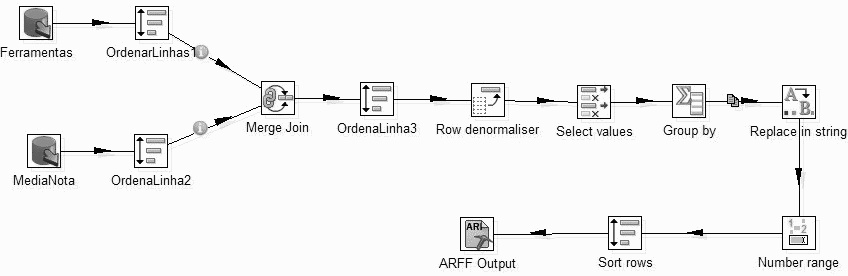
\includegraphics[width=.5\textwidth]{Pentaho.jpg}
\caption{Modelo gerado Pentaho Data Integration}
\label{fig:Pentaho}
\end{figure}

\section{Realizações dos experimentos}

\subsection{Objetivo}

O objetivo deste experimento foi analisar a utilização das ferramentas do AVA Moodle e relacionar com o desempenho acadêmico (média nota dos estudantes. Para realizar o experimento, foram utilizadas técnicas de mineração de dados e aplicação de questionário a fim de fazer um comparativo entre os dois métodos. 

\subsection{Aplicação e resultados dos algoritmos de mineração}

Conforme o procedimento descrito na seção 4, foi gerado o arquivo no formato ``.arff'', formato esse usado pelo software de mineração de dados Weka, que foi desenvolvido pela Universidade Waikato, e possui uma coleção de algoritmos de aprendizado de máquina para tarefas de mineração de dados. Os algoritmos podem ser aplicados diretamente a um conjunto de dados \cite{Weka:2014}. 

Após geração do arquivo, foi possível utilizar o WEKA para a aplicação do algoritmo de classificação J48 que é um algoritmo de árvore de decisão. As árvores de decisão são modelos estatísticos utilizados em problema de predição supervisionado, em que um conjunto de atributos é usado para predizer o valor de um atributo de saída (resultado), sendo o mapeamento destas entradas para as saídas denominadas de modelo preditivo\cite{Onoda:12}. Elas consistem em nodos que representam os atributos; de arcos, provenientes destes nodos e que recebem os valores possíveis para estes atributos; e de nodos folhas, que representam as diferentes classes de um conjunto de treinamento \cite{Shiba:13}. O resultado da execução da mineração de dados pode ser visualizado na figura ~\ref{fig:ResultJ48}. 
\begin{figure}[ht]
\centering
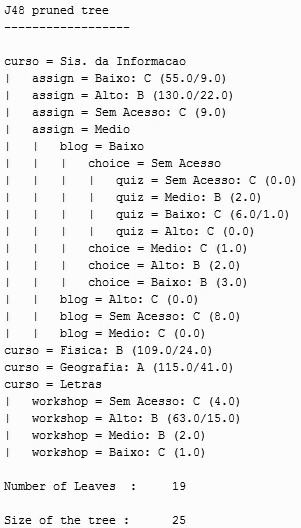
\includegraphics[width=.4\textwidth]{ResultJ48.jpg}
\caption{Resultado do algoritmo J48}
\label{fig:ResultJ48}
\end{figure}
A figura 2 mostra a saida do algoritmo J48, onde se interpreta que cada linha representa um nó da arvore. As linhas que possui o caractere ``{|}'' são filhos dos nós principais, e na proxima parte da linha é a regra. Após a regra encontra-se o resultado, a primeira parte dos valores entre parênteses indica quantas instâncias no conjunto estudado são corretamente classificados para este nó, e na segunda parte indica o número de instâncias incorretamente classificados. 

Diante desse resultado é possivel identificar como cada atributo se relaciona entre si, para alcançar o atributo meta, que no experimento foi o atributo ``MediaNota'' que corresponde a média das notas dos estudantes discretizadas como A,B,C como mostrado na seção 4. Na figura 2 é possivel identificar que o curso de Geografia tem as melhores médias das notas ``A'' com 115 instâncias corretamente classificadas corretamente e 41 instâncias classificadas incorretamente. O curso de Física foi classificado com tenho as médias das notas ``B'', já os cursos de Sistemas da Informação e Letras suas notas está variando de acordo com o uso de algumas ferramentas disponiveis no moodle. A ferramenta WEKA disponibiliza um resumo de alguns dados de medição de erro sobre o modelo gerado, através destas estatísticas geradas é possível identificar a quantidade de erros encontrados no conjunto de dados analisados como mostra a figura ~\ref{fig:ResumoJ48}.
\begin{figure}[ht]
\centering
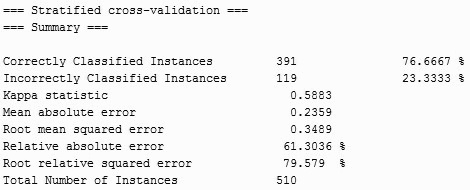
\includegraphics[width=.5\textwidth]{ResumoJ48.jpg}
\caption{Resumo do algoritmo J48}
\label{fig:ResumoJ48}
\end{figure}
Dentre os cursos escolhidos, nessa etapa foi possivel identificar as ferramentas e recursos mais utilizados pelos estudantes em cada curso no AVA Moodle. Como mostra a figura ~\ref{fig:MaisUsadas}, entre todas as ferramentas disponiveis o fórum e o envio e recebimento de arquivo (assign) são as ferramentas e recursos mais utilizados. 
\begin{figure}[ht]
\centering
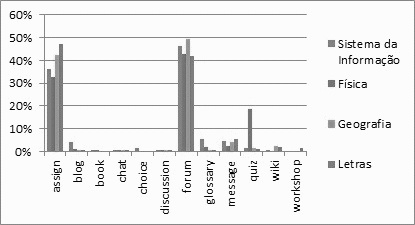
\includegraphics[width=.5\textwidth]{MaisUsadas.jpg}
\caption{Gráfico das Ferramentas mais usadas}
\label{fig:MaisUsadas}
\end{figure}

\subsection{Aplicação e resultados do questionário}

Em relação ao questionário, citado na seção dois, este foi elaborado em três partes. A primeira envolvendo perguntas relacionadas à disponibilidade de tempo dos tutores, a segunda parte teve como objetivo identificar o uso das ferramentas disponibilizadas pelo AVA Moodle e a terceira tem a finalidade de apontar o uso de outras ferramentas foram do AVA Moodle. O questionário foi aplicado com dezessete (17) tutores online, que atuam nos diversos cursos de graduação a distância da Universidade Federal de Alagoas (UFAL). O questionário apresentou dez (10) questões, cada questão com objetivo de entender um pouco sobre os tutores e as ferramentas que eles usam. A tabela 1 apresenta as perguntas do questionário. 
\begin{table}[!htpb]
 \centering
	\caption{Perguntas do questionário}
\begin{tabular}{|l|l|} \hline
\multicolumn{1}{|c|}{Enunciado das perguntas} & \multicolumn{1}{c|}{Alternativas} \\ \hline
\multirow{3}{9cm}{Há quanto tempo você é tutor?}  
& Primeiro semestre\\
& De dois a três semestre\\ 
& Mais de três semestre \\ \hline
\multirow{4}{9cm}{De quantas disciplinas você é tutor ao mesmo tempo?} 
& Uma única disciplina\\
& Duas \\
& Três \\
& Mais de três \\ \hline
\multirow{4}{9cm}{Onde geralmente você atende às demandas da tutoria?}
& Faculdade/Escola\\
& Trabalho \\
& Casa \\
& Outros \\ \hline
\multirow{4}{9cm}{O que você acha do tempo de resposta às dúvidas dos estudantes?}
& Tranquilo de atender\\
& Apertado mas realizável \\
& Bom \\
& Muito curto \\ \hline
\multirow{4}{9cm}{Considerando as necessidades dos alunos e a sua disponibilidade qual o prazo ideal para responder às dúvidas dos estudantes.}
& 24 Horas\\
& 48 Horas \\
& 72 Horas \\
& 96 Horas \\ \hline
\multirow{4}{9cm}{Qual a frequência de uso das ferramentas?(Blog, Book, Chat, Choice, Discussion, Forum, Glossary, Message, Quiz, Survey, Wiki, Workshop)}
& Nunca Usei\\
& Já usei \\
& Uso sempre em algumas disciplinas \\
& Uso Sempre \\ \hline
\multirow{4}{9cm}{Marque o nível de dificuldade encontrado por você em cada uma das ferramentas.(Blog, Book, Chat, Choice, Discussion, Forum, Glossary, Message, Quiz, Survey, Wiki, Workshop)}
& Nunca Usei\\
& Muito difícil \\
& Razoável\\
& Muito Fácil \\ \hline
\multirow{4}{9cm}{Aponte as dificuldades relatadas pelos estudantes nas ferramentas.}
& Nunca utilizaram\\
& Encontra dificuldade com frequência \\
& Alguns encontram \\
& Não encontram dificuldades \\ \hline
\multirow{2}{9cm}{Você utiliza alguma outra ferramenta fora do ambiente moodle? Quais?}
& Questão aberta \\
&  \\ \hline
\multirow{2}{9cm}{Na sua opinião o que você acha que poderia melhor no ensino a distância da UFAL?}
& Questão aberta\\
& \\ \hline	
\end{tabular}
\label{t_fixa}
\end{table}
A partir dos resultados do questionário foi possível chegar as seguintes conclusões. 

\begin{itemize}
	\item A primeira parte das perguntas foi direcionada a saber qual a disponibilidade do tutor em realizar as tarefas.  Onde foi possível identificar que não há     preocupação com relação ao tempo exigido para as realizações das tarefas direcionadas aos tutores. Levando e conta que o prazo exigido ao tutor para responder um estudante é de 48 hrs. Como podemos verificar na figura ~\ref{fig:ResultTempo}.
	\begin{figure}[ht]
\centering
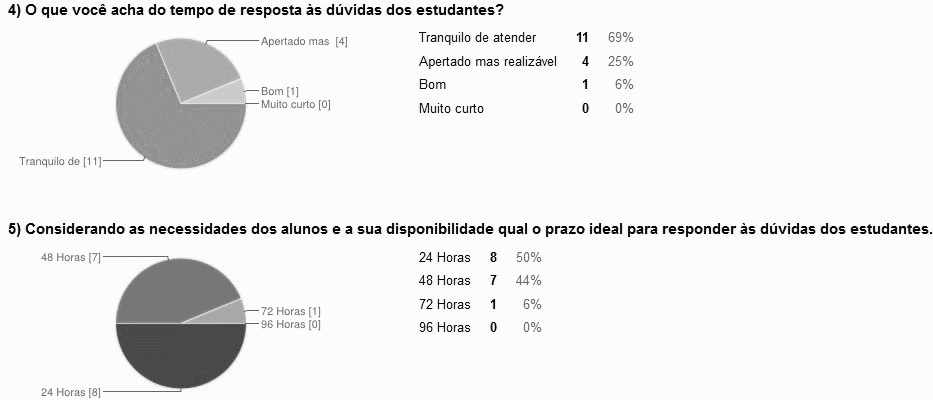
\includegraphics[width=.5\textwidth]{ResultTempo.jpg}
\caption{Gráfico relacionado ao tempo dos tutores}
\label{fig:ResultTempo}
\end{figure}
\item A segunda parte foi para identificar quais as ferramentas os tutores mais utilizam e se encontram alguma dificuldade no uso. De acordo com a pesquisa a ferramenta mais utilizada é o fórum com 81$\%$ das respostas afirmando que sempre usa a ferramenta. Apesar de não encontrarem nenhum tipo de dificuldade no uso de outras ferramentas. Como pode-se notar nas figuras abaixo.
	\begin{figure}[ht]
\centering
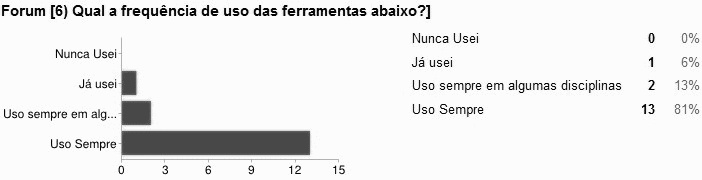
\includegraphics[width=.5\textwidth]{ResultForum.jpg}
\caption{Uso da ferramenta fórum}
\label{fig:ResultForum}
\end{figure}
	\begin{figure}[ht]
\centering
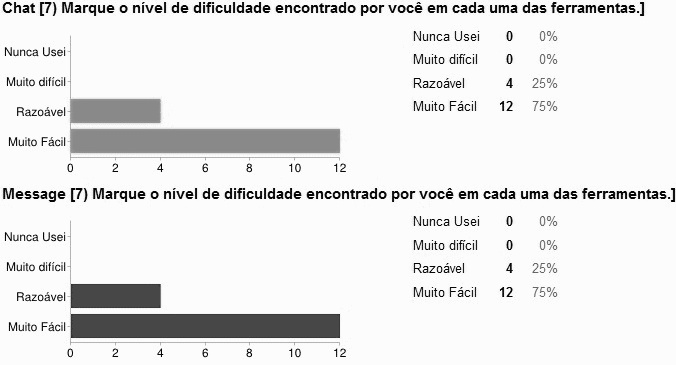
\includegraphics[width=.5\textwidth]{ResultDificuldade.jpg}
\caption{Dificuldade encontrada nas ferramentas}
\label{fig:Dificuldade}
\end{figure}
\item Por fim, foi possível verificar que apesar dos vários recursos e ferramentas disponível no AVA Moodle os tutores ainda utilizam ferramentas fora do ambiente o mais citado foi o uso do o e-mail como forma de comunicação entre os tutores e estudantes. 
\end{itemize}

Para mais detalhes o resultado completo do pesquisa foi disponibilizado no site www.....com.br.
\section{Resultados}

Analisando os resultados obtidos na seção 5.2 e 5.3 foi observado que tanto os resultados da aplicação de data mining quanto os resultados do questionário convergem para o mesmo ponto. Ou seja, apesar do AVA moodle disponibilizar uma série de ferramentas e recursos os mesmos são pouco utilizados. Dentre todas as ferramentas e recurso os mais utilizados são envio e recebimento de arquivos e o fórum e que atualmente essas ferramentas não estão tento muita influência no desempenho dos estudantes. 

O principal aspecto a ser destacado da seção 5.2, é mostrar que o desempenho dos estudantes não são influenciados pelo uso das ferramentas.  Podemos notar isso facilmente observado os dados do curso de geografia e física que mesmo tenho as melhores médias de notas não tem relação com o uso das ferramentas. Também nessa seção foi possível mostrar que a maioria das ferramentas não está sendo usada. 

Na seção 5.3, é importante mostrar que os tutores online realmente não usam ou não conhecem a maiorias das ferramentas, mesmo considerando de fácil uso. Vale a pena destacar que a maioria dos tutores (75$\%$ dos entrevistados) tem experiência, sendo tutor a mais de 3 semestre.

Os resultados apresentados nesse estudo atingiram o seu objetivo, evidenciando que a utilização das ferramentas no AVA moodle estão sendo subutilizadas.

\section{Conclusão e trabalhos futuros} 

A Educação a distância vem sendo cada dia mais utilizada pelas instituições de ensino, tanto para apoio aos cursos presenciais como para cursos à distância. Nesse cenário, uma ferramenta muito importante é o AVA. De acordo com a pesquisa realizada foi possível perceber que usuários do AVA Moodle quase não utilizam as ferramentas disponibilizadas no ambiente.

Os resultados obtidos nesse estudo apontam a viabilidade de realizar inferências relativas ao uso das ferramentas disponíveis no AVA Moodle. Estas inferências podem ser úteis para professores no sentido de ajuda-los no desenvolvimento de conteúdo e no processo de ensino e aprendizagem, aos tutores na intenção de auxilia-los no processo de avaliação e participação dos estudantes e aos alunos tornando mais motivados e presentes nos cursos EAD.

Como continuidade deste estudo, alguns pontos pendentes ainda deverão vir a ser considerados para a melhoria da pesquisa realizada, como os que se seguem: inserir novos algoritmos de classificação; aumentar a quantidade de amostras inserindo novos atributos e melhorado o processo de discretização dos dados; desenvolvimento do software capaz de auxiliar aos professores e tutores na escolha das ferramentas de acordo com o perfil do curso. 


\bibliographystyle{sbc}
\bibliography{sbc-template}

\end{document}
